% ==========================================
% PROJEKTPLANUNG
% ==========================================
\chapter{Projektplanung}

\section{Projektphasenmodell}

Das Projekt wurde nach einem sequenziellen Phasenmodell mit vier Hauptphasen strukturiert. 
Die Gesamtprojektdauer umfasste 80 Stunden und erstreckte sich über den Zeitraum vom 
1. Oktober 2025 bis zum 1. Dezember 2025. Jede Phase baute auf den Ergebnissen der vorherigen 
auf und war durch klar definierte Meilensteine abgegrenzt.

\subsection{Phasenübersicht}

Die folgende Tabelle~\ref{tab:phasenmodell} stellt die vier Projektphasen sowie deren Zeitanteile dar und dient als Grundlage für die detaillierte Ablauf- und Ressourcenplanung.

\begin{table}[H]
\centering
\footnotesize
\rowcolors{2}{EDAGDunkelgrau!10}{white}
\begin{tabularx}{\textwidth}{|p{3cm}|p{1.5cm}|X|}
\hline
\rowcolor{EDAGDunkelgrau!10}
\textbf{Phase} & \textbf{Dauer} & \textbf{Zentrale Aktivitäten} \\
\hline
Analysephase & 8h &
Erhebung des Projektumfelds, IST-Analyse, Strukturierung der Anforderungen, Prüfung datenschutzrelevanter Rahmenbedingungen \\
\hline
Planungsphase & 12h &
Entwurf der Systemarchitektur, Technologieauswahl, Definition des Datenmodells, Erstellung erster UI-Mockups, Wirtschaftlichkeitsbetrachtung \\
\hline
Durchführungsphase & 44h &
Aufsetzen der Entwicklungsumgebung, Implementierung der Datenbank- und Backendschicht, Umsetzung des Frontends, Systemintegration, Einrichtung der CI/CD-Pipeline \\
\hline
Abschlussphase & 16h &
Planung und Durchführung der Systemtests, Qualitätssicherung, Erstellung der technischen Dokumentation und Projektdokumentation \\
\hline
\rowcolor{EDAGDunkelgrau!30}
\textbf{Gesamt} & \textbf{80h} & \\
\hline
\end{tabularx}
\caption{Phasenmodell mit Zeitverteilung}
\label{tab:phasenmodell}
\end{table}

Die detaillierte Aufgliederung aller 21 Arbeitspakete mit zeitlichem Ablauf und Abhängigkeiten ist in Tabelle~\ref{tab:zeitplanung_detail} im Anhang dokumentiert.

\section{MVP-Definition und Priorisierung}

Das Projekt folgt dem \gls{mvp}-Ansatz, um innerhalb des begrenzten Zeitrahmens von 80 Stunden ein funktionsfähiges System zu liefern, das die kritischsten Anforderungen abdeckt.

\subsection{MVP-Kernfunktionen}

Die MVP-Definition fokussiert auf die wesentlichen Funktionen, die den größten Mehrwert für die Personalauswahl bieten:

\begin{table}[H]
\centering
\footnotesize
\rowcolors{2}{EDAGDunkelgrau!10}{white}
\begin{tabularx}{\textwidth}{|X|p{2cm}|p{3cm}|}
\hline
\rowcolor{EDAGDunkelgrau!10}
\textbf{Feature} & \textbf{Priorität} & \textbf{Begründung} \\
\hline
Mitarbeitersuche mit Skill-Filtern & Must-Have & Kernfunktion für Projektbesetzung \\
\hline
Profilverwaltung mit Skills & Must-Have & Datenbasis für Suche \\
\hline
Projektverwaltung (Manager) & Must-Have & Zentrale Dokumentation \\
\hline
Authentifizierung (OAuth2) & Must-Have & Sicherheitsanforderung \\
\hline
Rollenbasierte Zugriffskontrolle & Must-Have & Berechtigungskonzept \\
\hline
Dashboard mit Statistiken & Should-Have & Verbesserte UX \\
\hline
Activity-Logging & Should-Have & Audit-Trail \\
\hline
Stammdatenverwaltung (Admin) & Should-Have & Systemkonfiguration \\
\hline
\end{tabularx}
\caption{MVP-Feature-Priorisierung nach MoSCoW-Methode\cite{moscow_method}}
\label{tab:mvp_features}
\end{table}

\subsection{Abgrenzung: Nicht im MVP enthalten}

Folgende Features wurden bewusst für spätere Versionen zurückgestellt:

\begin{itemize}[noitemsep]
    \item \textbf{Skill-Gap-Analyse}: Automatische Identifikation fehlender Kompetenzen
    \item \textbf{Weiterbildungsempfehlungen}: KI-gestützte Trainingsvorschläge
    \item \textbf{Benachrichtigungssystem}: Push-Notifications und E-Mail-Alerts
    \item \textbf{Erweiterte Analytics}: Skill-Heatmaps, Trend-Analysen
    \item \textbf{Export-Funktionen}: PDF-Reports, Excel-Export
    \item \textbf{Integration mit Drittsystemen}: Jira, Confluence, LDAP
\end{itemize}

Diese Priorisierung stellt sicher, dass das \gls{mvp} innerhalb des Projektzeitraums vollständig funktionsfähig und testbar ist, während zukünftige Erweiterungen systematisch geplant werden können.

\subsection{Gantt-Diagramm}

Abbildung~\ref{fig:gantt} visualisiert den zeitlichen Ablauf des Projekts über acht Projektwochen mit den definierten Meilensteinen.

\begin{figure}[H]
\centering
\begin{ganttchart}[
    vgrid,
    hgrid,
    x unit=1.2cm,
    y unit title=0.7cm,
    y unit chart=0.6cm,
    title height=1,
    bar/.append style={fill=EDAGDunkelgrau!40},
    bar height=0.6,
    milestone/.append style={fill=EDAGRot!70, rounded corners=2pt},
    milestone height=0.6,
]{1}{8}

\gantttitle{Projektwochen (01.10.\,--\,01.12.2025)}{8} \\
\gantttitlelist{1,...,8}{1} \\

% Phasen
\ganttbar{Analysephase}{1}{1} \\
\ganttbar{Planungsphase}{2}{3} \\
\ganttbar{Durchführungsphase}{4}{6} \\
\ganttbar{Abschlussphase}{7}{7} \\
\ganttnewline
\vspace{0.3cm}

% Meilensteine
\ganttmilestone{M1: Anforderungen definiert}{1} \\
\ganttmilestone{M2: Architektur festgelegt}{2} \\
\ganttmilestone{M3: \gls{mvp} fertiggestellt}{6} \\
\ganttmilestone{M4: Projekt abgeschlossen}{7}

\end{ganttchart}
\caption{Gantt-Diagramm des Projektzeitplans}
\label{fig:gantt}
\end{figure}

\section{Ressourcenplanung}

Das Projekt wurde vom Auszubildenden Marvin Eschenbach durchgeführt mit Unterstützung des betrieblichen Betreuers Christian Henning (Beratung, Code-Reviews, Abnahme). Die Entwicklung erfolgte auf einem Entwicklungsrechner mit Docker- und Kubernetes-Unterstützung\cite{docker_docs,kubernetes_docs} sowie Zugriff auf die EDAG-Infrastruktur (Bitbucket\cite{bitbucket_docs}).

Sämtliche verwendeten Softwarewerkzeuge sind entweder Open Source oder unternehmensseitig lizenziert; zusätzliche Kosten entstehen dadurch nicht. Der vollständige Technologie-Stack ist in Tabelle~\ref{tab:technologien_detail} im Anhang dokumentiert.

\section{Wirtschaftlichkeitsbetrachtung}
\label{sec:wirtschaftlichkeit}

\subsection{Kostenplanung}

Die Projektumsetzung verursacht ausschließlich Personalkosten. Die notwendige Infrastruktur sowie alle Softwarewerkzeuge stehen bereits bereit. Die detaillierte Kostenaufstellung ist in Tabelle~\ref{tab:kosten_detail} dargestellt.

\begin{table}[H]
\centering
\footnotesize
\rowcolors{2}{EDAGDunkelgrau!10}{white}
\begin{tabularx}{\textwidth}{|p{5cm}|r|r|X|}
\hline
\rowcolor{EDAGDunkelgrau!10}
\textbf{Position} & \textbf{Stundensatz} & \textbf{Aufwand} & \textbf{Kosten} \\
\hline

\multicolumn{4}{|l|}{\textbf{Entwicklungskosten}} \\ \hline
Auszubildender (Entwicklung) & 35{,}00\,€\cite{azubi_stundensatz} & 70h & 2.450{,}00\,€ \\ \hline
Auszubildender (Dokumentation) & 35{,}00\,€\cite{azubi_stundensatz} & 10h & 350{,}00\,€ \\ \hline

\multicolumn{3}{|r|}{\textit{Zwischensumme Entwicklung}} & \textbf{2.800{,}00\,€} \\ \hline

\multicolumn{4}{|l|}{\textbf{Betreuung und Reviews}} \\ \hline
Projektbetreuer (Beratung) & 75{,}00\,€\cite{projektbetreuer_stundensatz} & 3h & 225{,}00\,€ \\ \hline
Projektbetreuer (Code-Reviews) & 75{,}00\,€\cite{projektbetreuer_stundensatz} & 2h & 150{,}00\,€ \\ \hline

\multicolumn{3}{|r|}{\textit{Zwischensumme Betreuung}} & \textbf{375{,}00\,€} \\ \hline

\multicolumn{4}{|l|}{\textbf{Infrastruktur (anteilig)}} \\ \hline
Entwicklungsrechner & -- & -- & 0{,}00\,€ \\ \hline
Softwarelizenzen & -- & -- & 0{,}00\,€ \\ \hline
Kubernetes-Infrastruktur & -- & -- & 0{,}00\,€ \\ \hline

\multicolumn{3}{|r|}{\textit{Zwischensumme Infrastruktur}} & \textbf{0{,}00\,€} \\ \hline

\rowcolor{EDAGDunkelgrau!30}
\multicolumn{3}{|r|}{\textbf{Gesamtinvestition}} & \textbf{3.175{,}00\,€} \\ \hline
\end{tabularx}
\caption{Detaillierte Kostenplanung}
\label{tab:kosten_detail}
\end{table}

\subsection{Make-or-Buy-Entscheidung}

Kommerzielle Skill-Management-Systeme kosten 5--15\,€ pro Nutzer/Monat\cite{skill_mgmt_market}, was bei 200 Mitarbeitern jährlich 12.000--36.000\,€ entspricht. Die Eigenentwicklung verursacht einmalig 3.175\,€.

Die \textbf{Make-Variante} wurde gewählt aufgrund: langfristig geringerer Kosten, vollständiger Datenkontrolle (DSGVO\cite{dsgvo}), optimaler Integration in EDAG-Infrastruktur und maximaler Flexibilität ohne Vendor-Abhängigkeit. Der detaillierte Vergleich findet sich in Tabelle~\ref{tab:make_or_buy_detail}.

\subsection{Nutzenanalyse}
\label{sec:nutzen_analyse}

Die Nutzenanalyse vergleicht den aktuellen manuellen Prozess (IST) mit dem automatisierten System (SOLL):

\textbf{IST-Prozess:} 2,5 Stunden pro Projektbesetzung = 125 Stunden/Jahr = 9.375\,€ Kosten\cite{projektbesetzung_aufwand,projektleiter_stundensatz}

\textbf{SOLL-Prozess:} 15 Minuten pro Projektbesetzung = 12,5 Stunden/Jahr = 937,50\,€ Kosten

\textbf{Einsparung:} 112,5 Stunden (90\%) = \textbf{8.437,50\,€ jährlich}

Die detaillierte Aufschlüsselung der Aktivitäten findet sich in den Tabellen~\ref{tab:ist_prozess_detail} und~\ref{tab:soll_prozess_detail} im Anhang.

\subsection{Amortisationsrechnung}
\label{sec:amortisation}

Die statische Amortisationsrechnung ermittelt den Zeitpunkt, zu dem die Investitionskosten durch eingesparte Kosten ausgeglichen sind:

\[
\text{Amortisationsdauer} = \frac{\text{Investitionskosten}}{\text{jährliche Einsparung}} = \frac{3.175\text{ EUR}}{8.437{,}50\text{ EUR}} = 0{,}38~\text{Jahre} \approx \textbf{4{,}5 Monate}
\]

Der \textbf{\gls{roi}} beträgt 166\% im ersten Jahr. Die Amortisation erfolgt bereits nach 4,5 Monaten.

\begin{figure}[H]
\centering
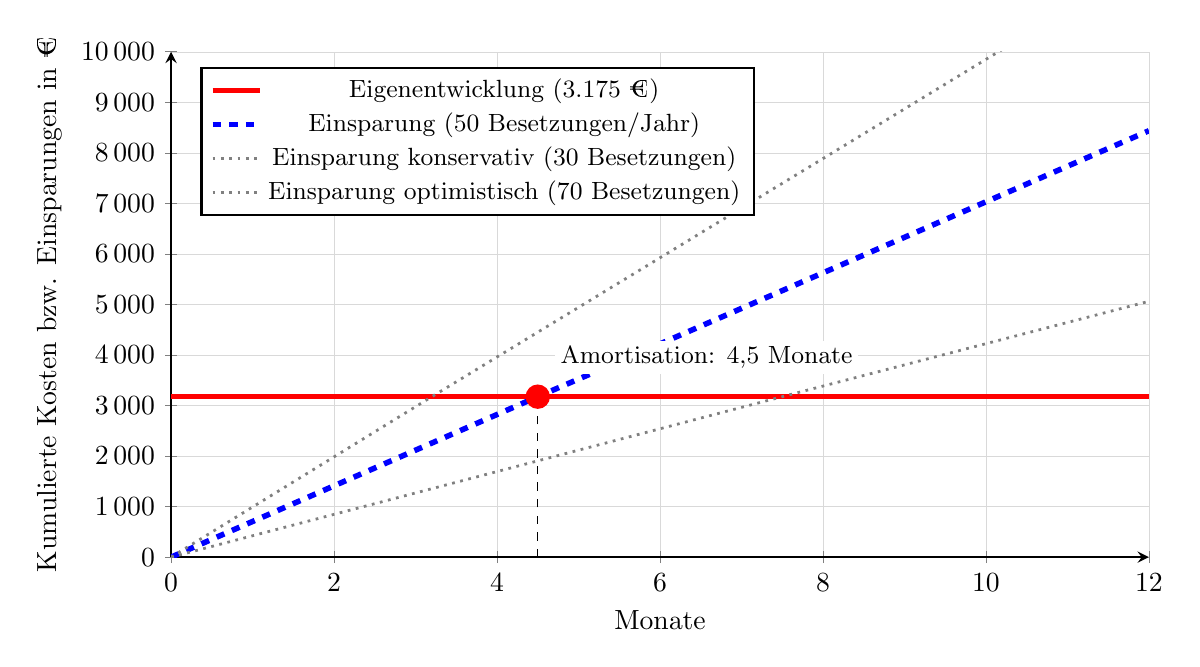
\begin{tikzpicture}
\begin{axis}[
    width=14cm,
    height=8cm,
    xlabel={Monate},
    ylabel={Kumulierte Kosten bzw. Einsparungen in €},
    xmin=0, xmax=12,
    ymin=0, ymax=10000,
    xtick={0,2,4,6,8,10,12},
    xticklabels={0,2,4,6,8,10,12},
    ytick={0,1000,2000,3000,4000,5000,6000,7000,8000,9000,10000},
    yticklabel style={/pgf/number format/fixed, /pgf/number format/1000 sep={\,}},
    scaled y ticks=false,
    grid=both,
    grid style={line width=.1pt, draw=gray!30},
    thick,
    legend pos=north west,
    legend style={font=\small},
    axis lines=left
]

% Eigenentwicklung (konstante Kosten)
\addplot[color=red, line width=2pt, mark=none] coordinates {
    (0, 3175) (12, 3175)
};
\addlegendentry{Eigenentwicklung (3.175~€)}

% Durchschnittliche Einsparung (50 Besetzungen/Jahr = 8437.50 EUR/Jahr)
\addplot[color=blue, line width=2pt, dashed, mark=none] coordinates {
    (0, 0) (4.5, 3175) (6, 4218.75) (12, 8437.50)
};
\addlegendentry{Einsparung (50 Besetzungen/Jahr)}

% Konservatives Szenario (30 Besetzungen/Jahr = 5062.50 EUR/Jahr)
\addplot[color=gray, line width=1pt, dotted, mark=none] coordinates {
    (0, 0) (7.5, 3175) (12, 5062.50)
};
\addlegendentry{Einsparung konservativ (30 Besetzungen)}

% Optimistisches Szenario (70 Besetzungen/Jahr = 11812.50 EUR/Jahr)
\addplot[color=gray, line width=1pt, dotted, mark=none] coordinates {
    (0, 0) (3.2, 3175) (12, 11812.50)
};
\addlegendentry{Einsparung optimistisch (70 Besetzungen)}

% Amortisationspunkt
\addplot[mark=*, only marks, mark size=4pt, color=red] coordinates {(4.5, 3175)};
\node[anchor=south west, font=\small, fill=white, inner sep=2pt] at (axis cs:4.7,3600) {Amortisation: 4,5 Monate};

% Break-Even Linie
\addplot[color=black, dashed, line width=0.5pt] coordinates {
    (4.5, 0) (4.5, 3175)
};

\end{axis}
\end{tikzpicture}
\caption{Amortisationsanalyse über 12 Monate}
\label{fig:amortisation}
\end{figure}

Selbst im konservativen Szenario (30 Besetzungen/Jahr) amortisiert sich die Investition nach 7,5 Monaten.
